%%%%%%%%%%%%%%%%%%%%%%%%%%%%%%%%%%%%%%%%%%%%%%%%%%%%%%%%%%%%%%%%%%%%%%%%%%%%%%%
% Author:  Pablo Alvarado
%
% Escuela de Ingeniería Electrónica
% Instituto Tecnológico de Costa Rica
%
% Tesis de Licenciatura
% 
% Phone:   +506 550 2106
% Fax:     +506 591 6629
% email:   palvarado@ietec.org
%
% $Id: main.tex 1513 2010-08-15 01:25:24Z palvarado $
%
%%%%%%%%%%%%%%%%%%%%%%%%%%%%%%%%%%%%%%%%%%%%%%%%%%%%%%%%%%%%%%%%%%%%%%%%%%%%%%%

%Modificado por Francis López Montero
%Listados:
% \begin{compactitem} 
% \item....
% \item....
% \item....
% \end{compactitem}

%Listados Numerados: 
% \begin{enumerate}
% \item....
% \item....
% \item....
% \end{enumerate}

%Voltear figuras:
%\begin{landscape}
%	\begin{figure}[b]
% 		\centering
%  		\includegraphics[width=1.5\textwidth]{Barrel_Shifter.pdf} %Imagenes en PDF no se degradan
%  		\caption{Diagrama de bloques del barrel shifter diseñado para la normalización de datos en el módulo de suma/resta de la FPU}
%  		\label{fig:bs}	
%	\end{figure}
%\end{landscape}

% \documentclass is book
\documentclass[12pt,twoside,letterpaper]{book}

\usepackage[utf8]{inputenc}
\usepackage{ifthen}                     % provide if-then-else operators

\usepackage{paralist} %fancy list of figures
\usepackage{multirow}
\usepackage{mathtools}
\usepackage{lscape}
\usepackage[shortlabels]{enumitem}
\usepackage[defaultlines=4,all]{nowidow}

\DeclareGraphicsExtensions{.png,.pdf,.jpg}
% --------------------------------------------------------------------------
% Global variables required in document formatting
% --------------------------------------------------------------------------
%
% BOOK MODE
%
\newboolean{bookmode}                  % boolean used to control book format
% Ensure that only one of the next two lines is active:
\setboolean{bookmode}{true}           % turn book mode on
%\setboolean{bookmode}{false}           % turn book mode off

%
% DRAFT MODE
%
\newboolean{draftmode}                  % boolean used to control draft-mode
% Ensure that only one of the next two lines is active:
\setboolean{draftmode}{true}            % turn draft mode on
%\setboolean{draftmode}{false}           % turn draft mode off
% --------------------------------------------------------------------------
%
% GENERAL AUTHOR, TITLE AND KEYWORDS
%
% Nombre del Estudiante
\newcommand{\scriptAuthor}{Nombre Apellido}

% Título de la tesis
\newcommand{\scriptTitle}{Diseño de ...} 

% Keywords
\newcommand{\scriptKeywords}{palabras, clave, ...}

% Descripción de la editorial
\newcommand{\boxeditorial}{%
}

% Para el PDF (cambiar si se desea otras cosas a lo indicado arriba
\newcommand{\pdfAuthor}{\scriptAuthor}
\newcommand{\pdfTitle}{\scriptTitle} 
\newcommand{\pdfKeywords}{\scriptKeywords}

% --------------------------------------------------------------------------

% include all packages and define all required general macros
%%%%%%%%%%%%%%%%%%%%%%%%%%%%%%%%%%%%%%%%%%%%%%%%%%%%%%%%%%%%%%%%%%%%%%%%%%%%%%%
% Author:  Pablo Alvarado
%
% Escuela de Electrónica
% Instituto Tecnológico de Costa Rica
%
% Phone:   +506 550 2106
% Fax:     +506 591 6629
% email:   palvarado@ietec.org
%
% $Id: macros.tex 1497 2010-08-09 17:04:26Z palvarado $
%
%%%%%%%%%%%%%%%%%%%%%%%%%%%%%%%%%%%%%%%%%%%%%%%%%%%%%%%%%%%%%%%%%%%%%%%%%%%%%%%

% Configuration of the exercises package, which is used to collect all
% problems and answers in the document.
\usepackage[exercisedelayed,answerdelayed,lastexercise]{exercise}
\renewcounter{Exercise}[chapter]
\renewcommand{\ExerciseName}{Problema}
\renewcommand{\theExercise}{\thechapter.\arabic{Exercise}}
\newcommand{\ExerciseLabel}{Exercise.\theExercise}
\renewcommand{\ExerciseHeader}%
{\textbf{\ExerciseName\ \theExercise.\ \ExerciseHeaderTitle\ }}
\renewcommand{\AnswerHeader}%
{\textbf{\ExerciseName\ \theExercise.\ }}


\usepackage{ifpdf}

% Command to change between draft or release mode:
\newcommand{\ifdraft}[2]{\ifthenelse{\boolean{draftmode}}{#1}{#2}}
% Command to change between draft or release mode:
\newcommand{\ifbook}[2]{\ifthenelse{\boolean{bookmode}}{#1}{#2}}

% include all required packages here
\usepackage[spanish,english]{babel}     % supports english, but default is 
                                        % spanish...
\newcommand*{\SelectSpanish}{%          % well, the last line indeed selects
  \hyphenrules{spanish}%                % english over spanish, but with this
  \languageshorthands{spanish}%         % command we turn it around.
  \captionsspanish                      % The reason: hyperref has some
  \datespanish                          % problems with the spanish babel,
}                                       % so we use some trick here so that it
\AtBeginDocument{\SelectSpanish}        % thinks it is english.

\usepackage{makeidx}                    % to create index file

\ifdraft{%
  %\usepackage[refpage]{nomencl}        % Use to easily administrate the list
 \usepackage{nomencl}                   % of symbols
}{%
 \usepackage{nomencl}
}
%\usepackage{times}                     % replace latex pk fonts with ps type I
                                        % don't forget to use dvips -D600 -Pcmz
                                        % to ensure Type I fonts!
\usepackage{amsmath}
\usepackage{amssymb,amstext}            % AMS-math and symbols package
\usepackage{mathrsfs}                   % Calygraphic fonts for transforms
\usepackage{array}                      % extensions to tabular environment
\usepackage{longtable}                  % supports extraordinary long tables
\usepackage{tabularx}                   % supports tables with fixed width
\usepackage{afterpage}                  % put something only after the page
\usepackage{multirow}                   % supports multiple row grouping in 
                                        % tables
\usepackage{multicol}                   % multiple columns environments
\usepackage{paralist}                   % a few enumeration settings

\usepackage[hang,%
            small,%
            bf]{caption}                % nicer figure captions
%\usepackage{sty/ftcap}                 % switch \abovecaptionskip and
%                                       % \belowcaptionskip for tables, in 
%                                       % order to avoid the caption to be
%                                       % too near to the table itself
% locally added packages
\usepackage{float}                      % really place figures "here" (H)
\usepackage{booktabs}                   % book type tabulars

% the own style with options depending on the draft mode
\ifdraft{%
\usepackage[todo]{sty/tecStyle}         % some command definitions
                                        % options [todo] todo-index
}{%
\usepackage{sty/tecStyle}               % some command definitions
                                        % options [todo] todo-index
}

%% fix the title for examples
\renewcommand{\examplelistname}{Índice de ejemplos}
\renewcommand{\examplename}{Ejemplo}

\renewcommand{\lstlistingname}{Código}% Listing -> Algorithm
%\renewcommand{\lstlistlistingname}{List of \lstlistingname s}% List of Listings -> List of Algorithms


\usepackage{url}                        % allows linebreaks at certain
                                        % characters or combinations of 
                                        % characters for URLs

\usepackage[nottoc]{tocbibind}          % Fix the hyperrefs to TOC,TOF, etc.
                                        % and ensure that they appear all in 
                                        % the Table of Contents

\usepackage{color}                      % Support for colors
\definecolor{dkred}{rgb}{0.5,0,0}       %   dark red
\definecolor{dkgreen}{rgb}{0,0.3,0}     %   dark green
\definecolor{dkblue}{rgb}{0,0.0,0.5}    %   dark blue
\definecolor{dkgray}{gray}{0.4}         %   dark gray
\definecolor{dkmagenta}{rgb}{0.3,0.0,0.3} % dark magenta
\definecolor{ltyellow}{rgb}{1.0,1.0,0.7}  % light yellow

\newcommand{\bG}[1]{\textcolor{dkgreen}{\textbf{#1}}}
\newcommand{\bR}[1]{\textcolor{dkred}{\textbf{#1}}}
\newcommand{\bB}[1]{\textcolor{dkblue}{\textbf{#1}}}
\newcommand{\bM}[1]{\textcolor{dkmagenta}{\textbf{#1}}}
\newcommand{\bY}[1]{\textcolor{dkyellow}{\textbf{#1}}}
\newcommand{\bC}[1]{\textcolor{dkcyan}{\textbf{#1}}}

% For pdflatex
% - The hyperref package should always be loaded last, since it has to
%   overwrite some of the commands.
% - The package subfigure caused that the pagebackrefs and index refs were set
%   incorrectly.

\ifpdf
%
% final / draft document options
\usepackage[pdftex,final]{graphicx}     % for inserting pdf-graphics.
                                        % options final / draft
\ifdraft{%

\usepackage[pdftex,%
            pdftitle={\pdfTitle},%
            pdfauthor={\pdfAuthor},%
            pdfsubject={Notas de Clase},%
            pdfkeywords={\pdfKeywords},%
            naturalnames=true,
            linktocpage,
            hyperindex,
            colorlinks,
            urlcolor=dkred,          %\href to external url
            filecolor=dkmagenta,     %\href to local file
            linkcolor=dkred,         %\ref and \pageref
            citecolor=dkgreen,       %\cite
            pagecolor=dkred,
            pagebackref,
            plainpages=false,
            pdfpagelabels,
            pdfpagemode=UseOutlines, % means use bookmarks (None,UseOutlines)
            % bookmarksopen=false,   % would show the whole hierarchy if true
            bookmarksnumbered=true,
            pdfpagelayout=OneColumn, % SinglePage,OneColumn,TwoColumnLeft,...
            pdfview=FitH, % FitB,FitBH,FitBV,Fit,FitH,FitV
            pdfstartview=FitH, % FitB,FitBH,FitBV,Fit,FitH,FitV
            ]{hyperref}
}{%
\usepackage[pdftex,%
            pdftitle={\pdfTitle},%
            pdfauthor={\pdfAuthor},%
            pdfsubject={Notas de clase},%
            pdfkeywords={\pdfKeywords},%
            naturalnames=true,
            linktocpage,hyperindex,
            colorlinks,
            urlcolor=dkred,          %\href to external url
            filecolor=dkmagenta,     %\href to local file
            linkcolor=dkred,         %\ref and \pageref
            citecolor=dkgreen,       %\cite
            pagecolor=dkred,
            % pagebackref,           % only in draft modus should this be on.
            plainpages=false,
            pdfpagelabels,
            pdfpagemode=UseOutlines, % means use bookmarks (None,UseOutlines)
            % bookmarksopen=false,   % open the whole hierarchy if true!
            bookmarksnumbered=true,
            pdfpagelayout=OneColumn, % SinglePage,OneColumn,TwoColumnLeft,...
            pdfview=FitH, % FitB,FitBH,FitBV,Fit,FitH,FitV
            pdfstartview=FitH, % FitB,FitBH,FitBV,Fit,FitH,FitV
            ]{hyperref}
}

%
% Ensure that the links of the images point to the top of the images and not
% to the caption
%
\usepackage[figure]{hypcap}

% %
% % Ensure that pdfLaTeX do the same spacing as LaTeX
% %
\pdfadjustspacing=1 
% %
\else   % i.e. if not pdf

\usepackage[active]{srcltx}             % insert links into the dvi to jump
\usepackage[dvips,final]{graphicx}      % for inserting eps-graphics.
                                        % options final / draft
                                        % into the sources directly.
\ifdraft{%
\usepackage[ps2pdf,%
            pdftitle={\pdfTitle}%
            pdfauthor={\pdfAuthor},%
            pdfsubject={Notas de clase},%
            pdfkeywords={\pdfKeywords},%
            % plainpages=false,
            linktocpage,
            hyperindex,
            pagebackref,
            % pdfpagelabels,
            pdfpagemode=UseOutlines,
            pdfstartview=FitH]{hyperref}
}{%
\usepackage[ps2pdf,%
            pdftitle={\pdfTitle}%
            pdfauthor={\pdfAuthor},%
            pdfsubject={Notas de clase},%
            pdfkeywords={\pdfKeywords},%
            % plainpages=false,
            linktocpage,
            hyperindex,
            % pagebackref,
            % pdfpagelabels,
            pdfpagemode=UseOutlines,
            pdfstartview=FitH]{hyperref}
}

%\usepackage[ps2pdf]{hyperref}

\fi  % end of if pdf or not

\usepackage{sty/algorithmic}            % algorithmic environment


\usepackage{rotating}                   % allow block rotation


%%%%%%%%%%%%%%%%%%%%%%%%%%%%%%%%%%%%%%%%%%%%%%%%%%%%%%%%%%%%%%%%%%%%%%%%%%%%%%%

%\sloppy

%
% Some own font definitions
%
\DeclareMathAlphabet{\mathpzc}{OT1}{pzc}{m}{it}
\DeclareMathAlphabet{\mathpss}{OT1}{cmss}{m}{sl}

%
% page layout
%

\usepackage{vmargin}
\setpapersize{USletter}

\ifbook{%
% left,top,right,bottom,headheight,headsep,footheight,footsep
%
% For the book legal-paper printing (two pages per legal paper)
\setmarginsrb{31mm}{8mm}{20mm}{7mm}{15pt}{15pt}{7mm}{9mm}
}{%
% For letter-paper printing
\setmarginsrb{33mm}{8mm}{23mm}{7mm}{15pt}{15pt}{7mm}{12mm}
}
%\setlength{\headheight}{15pt}         % fancy headers wanted this

%
% Fraction of Float Object / Text
%

\renewcommand{\topfraction}{0.95}       % how much of top of page should be 
                                        % allowed to be float object?
\renewcommand{\bottomfraction}{0.95}    % how much of bottom of page should be
                                        % allowed to be float object?
\renewcommand{\textfraction}{0.05}      % how much of page must be text?

\usepackage{fancyhdr}                   % fancy page headers

\usepackage{lastpage}

%
% header and footer layout (needs package fancyhdr)
%
\newcommand{\copyrightfooter}{\tiny{\copyright 2005-2010 --- P.~Alvarado %
    \qquad Uso exclusivo ITCR}}
%
\newcommand{\draftfoot}%
  {\ifdraft{\textcolor{dkblue}{\tiny\textsl{Borrador: \today}}{}}
           {}
}

\pagestyle{fancy}
\renewcommand{\chaptermark}[1]{\markboth{{\small
    \thechapter\hspace*{1mm}#1}}{}}
\renewcommand{\sectionmark}[1]{\markright{{\small
    \thesection\hspace*{1mm}#1}}{}}
\lhead[{\small\textbf\thepage}]{\fancyplain{}%
        {{\slshape \small\nouppercase{\leftmark}}}}
\chead[]{}
\rhead[\fancyplain{}%
        {{\slshape \small\nouppercase{\rightmark}}}]{{\small\textbf\thepage}}
\lfoot[]{\draftfoot}
\ifbook{%
  \cfoot[]{}
}{
  \cfoot[\copyrightfooter]{\copyrightfooter}
}
\rfoot[\draftfoot]{}
\renewcommand{\headrulewidth}{0.5pt}
\renewcommand{\footrulewidth}{0pt}

%
% Caption style for tables
% Requires the packages caption2 and ftcap
% (caption2 required this, but is obsolete now:)
%
%\newcaptionstyle{tablecaptionstyle}{%
%  \renewcommand\captionlabelfont{\normalsize\bf}
%  \renewcommand\captionfont{\normalsize}
%  \usecaptionstyle{hang}%
%}

% For caption v3:
\captionsetup[table]{position=top,format=hang,textfont={normalsize},labelfont={normalsize,bf}}

\newcommand{\tablecaption}[2][foo]{%
  \ifthenelse{\equal{#1}{foo}}{%
    %\captionstyle{tablecaptionstyle}%
    \caption{#2}%
  }
  {%
    %\captionstyle{tablecaptionstyle}%
    \caption[#1]{#2}%
  }
}
\addto\extrasspanish{\renewcommand{\tablename}{Tabla}}
\addto\extrasspanish{\renewcommand{\listtablename}{\'Indice de tablas}}

%
% paragraph layout
%
\renewcommand{\baselinestretch}{1.1}    % line spacing
\parindent0em                           % indentation width of first line
\parskip1.3ex                           % space between paragraphs

%
% document consists of
% chapter - section - subsection - subsubsection - paragraph - subparagraph
%
\setcounter{secnumdepth}{2}             % depth of section numbering
\setcounter{tocdepth}{2}                % depth of table of contents

%
% prepares index from entries like \index{word} or \index{group!word}.
% don't forget to call "makeindex filename" for final index generation.
%
\makeindex                            %% for package makeidx.sty
%\newindex{default}{idx}{ind}{Index}  %% for package index.sty

\newcommand{\octave}{GNU/Octave}


%
% prepares notation or nomenclature 
%
%\makeglossary
\makenomenclature

%%% Local Variables: 
%%% mode: latex
%%% TeX-master: "main"
%%% End: 


% allow equations to be splitted (breaked) into several pages
\allowdisplaybreaks[3]

% --------------------------------------------------------------------------
\begin{document}
  % where to look for graphics
  \graphicspath{{./}{./fig/}}

  \pagenumbering{alph}
  % fix some terms not activated due to the bug of hyperref with spanish.
  \renewcommand{\tablename}{Tabla}
  \renewcommand{\listtablename}{\'Indice de tablas}
  \renewcommand{\examplesolution}{Solución}
  \pagestyle{empty}

  %% ---------------------------------------------------------------------------
%% titlepage.tex
%%
%% Title page
%%
%% $Id: titlepage.tex 1452 2010-07-07 00:55:16Z palvarado $
%% ---------------------------------------------------------------------------

\thispagestyle{empty} 

\begin{center}

Tecnológico de Costa Rica

\par\vspace{1ex}

Escuela de Ingeniería Electrónica

\par\vspace{20mm}


\includegraphics[width=20mm]{TEC}

\par\vspace*{\fill}

{\large\bf{\scriptTitle}}

\par\vspace*{\fill}

Informe de Proyecto de Graduación para optar por el título de

Ingeniero en Electrónica con el grado académico de Licenciatura

\par\vspace{20mm}

\scriptAuthor

\vspace*{\fill}

\ifdraft{%
{Borrador de \today}
}{
Versión de \today
}
\end{center}
\newpage 
\cleardoublepage 


%%% Local Variables: 
%%% mode: latex
%%% TeX-master: "main"
%%% End: 
                                 % Titlepage
  \thispagestyle{empty}

\rule{10mm}{0pt}

\vfill

Declaro que el presente Proyecto de Graduación ha sido realizado enteramente
por mi persona, utilizando y aplicando literatura referente al tema e
introduciendo conocimientos propios.

En los casos en que he utilizado bibliografía he procedido a indicar las
fuentes mediante las respectivas citas bibliográficas.  En consecuencia,
asumo la responsabilidad total por el trabajo de graduación realizado y por
el contenido del correspondiente informe final.



\vspace*{8mm}

\begin{flushright}
  \scriptAuthor\par
  Cartago, \today\par
  Céd: 1-0123-0456
\end{flushright}

\cleardoublepage

%%% Local Variables: 
%%% mode: latex
%%% TeX-master: "main"
%%% End: 

  \chapter*{Resumen}
\thispagestyle{empty}

El resumen es la síntesis de lo que aparecerá en el tesis. Tiene que ser lo
suficientemente consiso y claro para que alguien que lo lea sepa qué esperar
del resto de la tesis si la leyera completamente. Puede concluir con palabras
clave, que son los temas principales tratados en el documento. El resumen queda
fuera de la numeración del resto de secciones.

No se acostumbra utilizar referencias bibliográficas, tablas, o figuras
en el resumen.

\bigskip

\textbf{Palabras clave:} \scriptKeywords

\clearpage
\chapter*{Abstract}
\thispagestyle{empty}

The same as before, but in English.

\bigskip

\textbf{Keywords:} word 1, word 2, 

\cleardoublepage

%%% Local Variables: 
%%% mode: latex
%%% TeX-master: "main"
%%% End: 

  \vspace*{0.4\textheight}
{\hfill{\Large{\emph{a mis queridos padres}}}}

  \chapter*{Agradecimientos}
\thispagestyle{empty}

A mis padres que han sido el pilar fundamental en mi vida, ustedes son los responsables de que sea la persona que soy. Gracias por sus sabios consejos y apoyo incondicional.

A mi hermano Rolando, quien ha sido un gran apoyo en todos mis proyectos, siempre un ejemplo para mí, y mi modelo a seguir mientras crecía.

A mi primo Miguel por ser mi paño de lágrimas siempre que necesité dinero para continuar con mis proyectos, gracias por brindarme tu apoyo en todas mis metas.

Al Ing. Dr. Alfonso Chacón Rodríguez por toda la colaboración que me brindó, no sólo para que este proyecto se consolidase, sino por toda su ayuda para que pudiese continuar estudiando en esta institución. Gracias por sus consejos, sus duras lecciones y amistad.

Finalmente a los Ingenieros: Dr.  Juan Agustín Rodríguez quien sentó las bases para poder llevar a cabo este proyecto, al M.Sc. Carlos Salazar y M.Sc. Ronny Gracía, quienes colaboraron en la supervisión para que este proyecto fuese exitoso.







\vspace*{1cm}

\scriptAuthor

Cartago, \today

\cleardoublepage

%%% Local Variables: 
%%% mode: latex
%%% TeX-master: "paMain"
%%% End: 


  %----------------------------------------------------------------------------
  \frontmatter
  %----------------------------------------------------------------------------
  \pagestyle{fancy}

  \pdfbookmark[1]{Indice General}{Indice General}

  \parskip0ex                           % space between paragraphs

  \tableofcontents                                      % Table of contents
  \listoffigures                                        % List of figures
  \listoftables                                         % List of tables

\ifdraft{%
  % todo's                                              % TODOs
  \listoftodo
}{%
}

  %% ---------------------------------------------------------------------------
%% paNotation.tex
%%
%% Notation
%%
%% $Id: notation.tex 1467 2010-07-24 16:47:17Z palvarado $
%% ---------------------------------------------------------------------------

\newcommand{\nms}{\negmedspace}

%%
% Commands required for the nomenclature groups
%
% There are following prefix forms:
%  a   abbreviation    \syma[key]{symbol}{description}
%  g   general         \symg[key]{symbol}{description}
%%

\newcommand{\nmstyle}[1]{\large\item[\textbf{#1}]\normalsize}

\renewcommand{\nomgroup}[1]{%
  \ifthenelse{\equal{#1}{A}}{\nmstyle{Abreviaciones}\normalsize}{%
  \ifthenelse{\equal{#1}{G}}{\bigskip\nmstyle{Notación general}\normalsize}%
  }
}

\newcommand{\syma}[3][foo]{%
  \ifthenelse{\equal{#1}{foo}}%
  {\nomenclature[A#2\ ]{#2}{#3}}{\nomenclature[A#1\ ]{#2}{#3}}}
\newcommand{\symg}[3][foo]{%
  \ifthenelse{\equal{#1}{foo}}%
  {\nomenclature[G#2\ ]{#2}{#3}}{\nomenclature[G#1\ ]{#2}{#3}}}

%%
% Command definitions for localized symbol format definition
%%
\renewcommand{\Re}{\operatorname{Re}}
\renewcommand{\Im}{\operatorname{Im}}

\newcommand{\prt}[1]{\ensuremath{\mathcal{#1}}}         %% partitioning
\newcommand{\img}[1]{\ensuremath{\mathcal{#1}}}         %% image as a set
\newcommand{\reg}[1][R]{\ensuremath{\mathcal{#1}}}      %% region
\newcommand{\pred}[1]{\ensuremath{\mathrm{#1}}}         %% predicate
\newcommand{\operat}[2]{\mathcal{#1}\left\{#2\right\}}
\newcommand{\transf}[1]{\mathscr{#1}}
\newcommand{\fourier}[1]{\transf{F}\left\{#1\right\}}
\newcommand{\ifourier}[1]{\transf{F}^{-1}\left\{#1\right\}}
\newcommand{\laplace}[1]{\transf{L}\left\{#1\right\}}
\newcommand{\ulaplace}[1]{\transf{L}_u\left\{#1\right\}}
\newcommand{\blaplace}[1]{\transf{L}_b\left\{#1\right\}}
\newcommand{\ilaplace}[1]{\transf{L}^{-1}\left\{#1\right\}}
\newcommand{\ztrans}[1]{\transf{Z}\left\{#1\right\}}
\newcommand{\iztrans}[1]{\transf{Z}^{-1}\left\{#1\right\}}
\newcommand{\zutrans}[1]{\transf{Z}_u\left\{#1\right\}}
\newcommand{\exceq}{\ensuremath{\overset{!}{=}}}

\newcommand{\signum}{\operatorname{signum}}
\newcommand{\vct}[1]{\ensuremath{\underline{\mathbf{#1}}}}
\newcommand{\mat}[1]{\ensuremath{\mathbf{#1}}}
\newcommand{\vctmu}{\vct{\boldsymbol{\mu}}}
\newcommand{\vctzeta}{\vct{\boldsymbol{\zeta}}}
\newcommand{\vctpi}{\vct{\boldsymbol{\pi}}}
\newcommand{\vctvarphi}{\vct{\boldsymbol{\varphi}}}
\newcommand{\raum}[1]{\ensuremath{\mathbb{#1}}}
\newcommand{\matSigma}{\mat{\boldsymbol{\Sigma}}}
\newcommand{\matLambda}{\mat{\boldsymbol{\Lambda}}}
\newcommand{\matPsi}{\mat{\boldsymbol{\Psi}}}
\newcommand{\matPhi}{\mat{\boldsymbol{\Phi}}}
\newcommand{\row}[2]{\ensuremath{\mathbf{\underline{#1}_{#2(\cdot)}}}}
\newcommand{\col}[2]{\ensuremath{\mathbf{\underline{#1}_{(\cdot) #2}}}}
\newcommand{\seq}[1]{\ensuremath{#1}}
\newcommand{\set}[1]{\ensuremath{\mathcal{#1}}}
\newcommand{\gset}[1]{\ensuremath{#1}} %% set for greek symbols
\newcommand{\front}[1]{\widehat{\set{#1}}}
\newcommand{\setlambda}{\set{\boldsymbol{\lambda}}}
\newcommand{\klass}[1]{\ensuremath{\mathpss{#1}}}
\newcommand{\graph}[1]{\ensuremath{\mathsf{#1}}}
\newcommand{\lab}[1]{\ensuremath{\mathpss{L}(#1)}}
\newcommand{\myfrac}[2]{{\footnotesize #1/#2}}
\newcommand{\ifthenspc}{\rule{3mm}{0mm}}
\newcommand{\point}[1]{\ensuremath{\mathsf{#1}}}
\newcommand{\estim}[1]{\ensuremath{\hat{#1}}}
\newcommand{\numset}[1]{\ensuremath{\mathbb{#1}}}
\newcommand{\tuple}[1]{\ensuremath{\left\langle#1\right\rangle}}
\newcommand{\conj}[1]{\ensuremath{{{#1}^{\ast}}}}
\newcommand{\base}[1]{\set{#1}}
\newcommand{\zeron}[1]{\ensuremath{\underset{\uparrow}{#1}}}
\newcommand{\sysT}{\ensuremath{\mathcal{T}}}
\newcommand{\sys}[1]{\ensuremath{\sysT\left[#1\right]}}
\newcommand{\sen}{\operatorname{sen}} % sinus in spanish (seno)
\newcommand{\senh}{\operatorname{senh}} % sinus hiperbolicus in spanish (seno)
\newcommand{\arcsen}{\operatorname{arcsen}} % arcus sinus hiperbolicus in spanish (arcoseno)
\newcommand{\sgn}{\operatorname{sgn}} % signus
\newcommand{\roc}{\text{ROC: }}

\newcommand{\code}[1]{\texttt{#1}}
\newcommand{\conv}{\ensuremath{\ast}}
\newcommand{\cconv}{\ensuremath{\;\,\text{\footnotesize{N}}\!\!\!\!\!\!\bigcirc}}
\newcommand{\Ln}{\operatorname{Ln}}
\newcommand{\sa}{\operatorname{sa}}
\newcommand{\senc}{\operatorname{senc}}
\newcommand{\si}{\operatorname{si}}


%% Natural, Integer and Real Numbers
\newcommand{\setA}{\ensuremath{\mathbb{A}}}
\newcommand{\setB}{\ensuremath{\mathrm{I\negthinspace B}}}
\newcommand{\setC}{\ensuremath{\mathbb{C}}}
\newcommand{\setD}{\ensuremath{\mathrm{I\negthinspace D}}}
\newcommand{\setE}{\ensuremath{\mathrm{I\negthinspace E}}}
\newcommand{\setF}{\ensuremath{\mathrm{I\negthinspace F}}}
\newcommand{\setG}{\ensuremath{\mathbb{G}}}
\newcommand{\setH}{\ensuremath{\mathrm{I\negthinspace H}}}
\newcommand{\setI}{\ensuremath{\mathbb{I}}}
\newcommand{\setJ}{\ensuremath{\mathbb{J}}}
\newcommand{\setK}{\ensuremath{\mathrm{I\negthinspace K}}}
\newcommand{\setL}{\ensuremath{\mathrm{I\negthinspace L}}}
\newcommand{\setM}{\ensuremath{\mathrm{I\negthinspace M}}}
\newcommand{\setN}{\ensuremath{\mathrm{I\negthinspace N}}}
\newcommand{\setO}{\ensuremath{\mathbb{O}}}
\newcommand{\setP}{\ensuremath{\mathrm{I\negthinspace P}}}
\newcommand{\setQ}{\ensuremath{\mathbb{Q}}}
\newcommand{\setR}{\ensuremath{\mathrm{I\negthinspace R}}}
\newcommand{\setS}{\ensuremath{\mathbb{S}}}
\newcommand{\setT}{\ensuremath{\mathbb{T}}}
\newcommand{\setU}{\ensuremath{\mathbb{U}}}
\newcommand{\setV}{\ensuremath{\mathbb{V}}}
\newcommand{\setW}{\ensuremath{\mathbb{W}}}
\newcommand{\setX}{\ensuremath{\mathbb{X}}}
\newcommand{\setY}{\ensuremath{\mathbb{Y}}}
\newcommand{\setZ}{\ensuremath{\mathbb{Z}}}


%%
% Multimap symbols
%
\newcommand{\ttoF}{\,\circ\!\negthickspace\longrightarrow\negthickspace\!\negthickspace\bullet\,}
\newcommand{\Ftot}{\,\bullet\negthickspace\!\negthickspace\longleftarrow\!\negthickspace\circ\,}
\newcommand{\ttoZ}{\ttoF}
\newcommand{\Ztot}{\Ftot}
\newcommand{\ttoZu}{\overset{z_u}{\ttoF}}
\newcommand{\Zutot}{\overset{z_u}{\Ftot}}
\newcommand{\vttoF}{\text{\begin{sideways}$\Ftot$\end{sideways}}}
\newcommand{\vFtot}{\text{\begin{sideways}$\ttoF$\end{sideways}}}
\newcommand{\vttoZ}{\vttoF}
\newcommand{\vZtot}{\vFtot}
\newcommand{\ttoDF}{\underset{N}{\ttoF}}
\newcommand{\DFtot}{\underset{N}{\Ftot}}

\newcommand{\thisis}[2]{\underset{#1}{\underbrace{#2}}}

%%% Local Variables:
%%% mode: latex
%%% TeX-master: "paMain"
%%% End:
                                    % Notation
  %% ---------------------------------------------------------------------------
%% paNotation.tex
%%
%% Notation
%%
%% $Id: paNotation.tex,v 1.15 2004/03/30 05:55:59 alvarado Exp $
%% ---------------------------------------------------------------------------

\cleardoublepage
\renewcommand{\nomname}{Lista de símbolos y abreviaciones}
\markboth{\nomname}{\nomname}
\renewcommand{\nompreamble}{\addcontentsline{toc}{chapter}{\nomname}%
\setlength{\nomitemsep}{-\parsep}
\setlength{\itemsep}{10ex}
}

%%
% Símbolos en la notación general
% (es posible poner la declaración en el texto
%%

% \symg[t]{$\sys{\cdot}$}{Transformación realizada por un sistema}
% \symg[yscalar]{$y$}{Escalar.}
% \symg[zconjugado]{$\conj{z}$}{Complejo conjugado de $z$}
% \symg[rcomplexreal]{$\Re(z)$ o $z_{\Re}$}{Parte real del número complejo $z$}
% \symg[icompleximag]{$\Im(z)$ o $z_{\Im}$}{Parte imaginaria del número
%                                         complejo $z$}
% \symg[jimaginario]{$j$}{$j=\sqrt{-1}$}
% \symg[xvector]{$\vct{x}$}{Vector. \newline\hspace{1mm}%
%   $\vct{x}=\left[ x_1 \; x_2 \; \ldots \; x_n \right]^T =
%   \begin{bmatrix}
%     x_1 \\ x_2 \\ \vdots \\ x_n
%   \end{bmatrix}$}

% \symg[amatrix]{$\mat{A}$}{Matriz. \newline\hspace{1mm}%
%   $\mat{A} =
%   \begin{bmatrix}
%     a_{11} & a_{12} & \cdots & a_{1m}\\
%     a_{21} & a_{22} & \cdots & a_{2m}\\
%     \vdots & \vdots & \ddots & \vdots\\
%     a_{n1} & a_{n2} & \cdots & a_{nm}\\
%   \end{bmatrix}$}

% \symg[C]{$\setC$}{Conjunto de los números complejos.}

%%
% Algunas abreviaciones
%%

\syma{DCILab}{Laboratorio de Diseño de Circuitos Integrados}
\syma{RIS}{Redes Inalámbricas de Sensores}
\syma{FPGA}{Arreglo de Compuertas Programables}
\syma{SiRPA}{Sistema de Reconocimiento de Patrones Acústicos}
\syma{HDL}{Lenguaje de Descripción de Hardware}
\syma{SoC}{Sistema integrado en un chip}
\syma{ASIC}{Circuito Integrado de Aplicación Específica}
\syma{MOSIS}{Servicios de Implementación, Metal, Óxido, Semiconductor}
\syma{EDA}{Automatización de Diseño Electrónico}
%\syma{Script}{Archivo que contiene un conjunto de órdenes e instrucciones, que implementan una función de forma programática.}
\syma{ICs}{Circuitos Integrados}
\syma{CBIC}{Circuito Integrado basado en celdas estándar}
\syma{IP Core}{Bloque de propiedad intelectual}
\syma{GL, GLD, GLN}{Gate level description/netlist: metodología para describir hardware asociando la codificación a nivel de compuertas y registros de una tecnología en particular}
\syma{RTL}{Sub-dependencia de los lenguajes de descripción de hardware usada para la descripción de lógica secuencial. Comúnmente usada para referirse a la codificación en un lenguaje de descripción de hardware}
\syma{STA}{Análisis de tiempo estático. Corresponde a la metodología mediante la cual se analiza el desempeño de un diseño en términos de sincronía de señales.}
\syma{ICT}{Instituto Costarricense de Turismo}
\syma{ITCR}{Instituto Tecnológico de Costa Rica}
\syma{FPU}{Unidad de punto flotante}
\syma{HMM}{Modelos Ocultos de Marcov}
\syma{TCL}{Tool Command Language, lenguaje de comandos de herramientas, acrónimo para referir al lenguaje interpretado "tickle"}
\printnomenclature[20mm]

%%% Local Variables:
%%% mode: latex
%%% TeX-master: "paMain"
%%% End:
                                    % Abbreviation

  \parskip1.3ex                           % space between paragraphs

  %----------------------------------------------------------------------------
  \mainmatter
  %----------------------------------------------------------------------------
  % where to look for graphics
  \graphicspath{{./}{./fig/}}

  % Main files
  %% ---------------------------------------------------------------------------
%% intro.tex
%%
%% Introduction
%%
%% $Id: intro.tex 1477 2010-07-28 21:34:43Z palvarado $
%% ---------------------------------------------------------------------------

\chapter{Introducción}
\label{chp:intro}
\section{Entorno de la tesis}

Costa Rica es uno de los países que se encuentran a la vanguardia en materia de conservación ambiental, esto debido al sistema de áreas protegidas, cerca del 25\% del territorio nacional cuenta con alguna categoría de protección. Las políticas nacionales de protección no sólo abogan por preservar la flora y fauna local sino también por mantener un desarrollo sostenible garantizando la perpetuidad de los recursos naturales. \cite{website:sinac}

Los recursos naturales son, innegablemente, el medio fundamental para el crecimiento integral de las sociedades modernas. Estos se encuentran implícitos en todas las actividades humanas y son indispensables para sostener el estilo de vida del ciudadano moderno, desde su nutrición, materia prima para la manufactura de la tecnología que emplea, los servicios que recibe, entre otros. \cite{website:inbio}

Por otra parte la riqueza natural representa una gran fuente de ingresos económicos para el país, debido al turismo. Según el informe del ICT, durante el primer trimestre del 2015 al país arribaron por todas las vías de ingreso un total de 811,379 personas, para el primer trimestre del 2016 arribaron un total de 919,624 lo que representa un incremento del 13.3\%. \cite{website:ict}

No obstante al marco jurídico en materia ambiental y los programas de protección ambiental hacia la flora y fauna, Costa Rica tiene serios problemas de caza furtiva y tala indiscriminada, pues los programas de conservación y la legislación actual son insuficientes para velar por la correcta protección de los recursos naturales (i.e. flora, fauna, minerales, etc), en mayor medida debido a la carencia de los fondos y personal necesarios para ejercer con más rigurosidad las políticas de conservación y penalización. De forma ilustrativa según el Sistema Nacional de Áreas de Conservación, en el 2014 eran necesarios, aproximadamente, 300 funcionarios dedicados al control y protección de las áreas protegidas (i.e. guardabosques) y el Estado era incapaz de hacer las contrataciones por falta de presupuesto. \cite{website:sinac}

Dado el dilema expuesto, estatalmente, se han puesto en marcha diversas estrategias para enfrentar la problemática; sin embargo, aumentar el recurso humano no es la opción más rentable para el Estado, siendo probable que una densidad mayor de guardabosques tampoco sea la solución. Partiendo de estas premisas se ha optado por un cambio de visión en camino a resolver el problema. Se considera que la posible solución resida en el uso de tecnología para facilitar la labor de los guardabosques.

Esta propuesta de solución tecnológica consiste en la implementación de una \textit{RIS} \footnote{\textit{RIS}: Acrónimo en español para Red Inalámbrica de Sensores} para vigilar de forma remota las zonas protegidas. Una \textit{RIS} no es otra cosa que una serie de dispositivos autónomos distribuidos en un área de interés, utilizando elementos de instrumentación (i.e. sensores) para monitorear condiciones físicas o ambientales. Cada miembro de la red corresponde a un nodo \cite{website:ni}. Se considera que si la \textit{RIS} no es la solución más viable, es una solución muy eficiente ya que las \textit{RIS} son capaces de medir parámetros, almacenarlos, procesarlos y enviarlos entre sí, lo cual permite ejecutar muchas de las labores realizables por un guardabosques. Como consideración especial, debe tenerse en cuenta que en un bosque no hay un acceso fácil a fuentes de alimentación eléctrica, por lo que es imperativo que la \textit{RIS} tenga un bajo consumo energético.

En respuesta a esta restricción, se presenta el proyecto: "Sonidos Ilegales" \cite{website:dcilab} de la Escuela de Ingeniería Electrónica del \textit{ITCR} \footnote{Instituto Tecnológico de Costa Rica} el cual refiere a la implementación de un sistema de reconocimiento de sonidos de motosierras, disparos de armas de fuego, como indicadores indirectos de actividades de tala y caza ilegales en zonas protegidas. Este proyecto consiste en el diseño de un sistema de hardware \textit{SoC} \footnote{SoC: Single on Chip. Sistema integrado en un chip} de bajo consumo energético el cual lleva a cabo las operaciones de procesamientos mencionas de la \textit{RIS}. \cite{website:inv_esc_electro, sirpa_SoC} 

El funcionamiento de una \textit{RIS} consiste en la obtención de muestras de señales
acústicas del medio, que en este caso se trata de un bosque. Seguidamente, los datos son iprocesados aplicando reconocimiento de patrones. En caso de encontrar un estado de alarma: disparo o motosierra, se activara el bloque de transmisión de información donde posteriormente la persona a cargo de la protección de la zona (el guardabosques), recibirá una notificación donde se le indicará el tipo de suceso y en cual nodo de la red se hizo de detección. En la figura \ref{nodoRIS} se muestra un diagrama de bloques de un nodo de la RIS que permite, a groso modo, entender el funcionamiento de la misma. \nocite{Carlosthesis}

\begin{figure}[h]
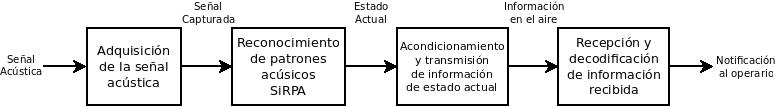
\includegraphics[width=\textwidth]{Nodo_RIS.jpeg}
\centering
\caption{Procesamiento realizado por cada nodo miembro de la RIS \cite{Jordanthesis}}
\label{nodoRIS}
\end{figure}


Interiorizando en la unidad de procesamiento, específicamente en el bloque denominado \textit{SiRPA} \footnote{SiRPA, es el acrónimo en español para Sistema de Reconocimiento de Patrones Acústicos}, este sigue una estructura estándar de un sistema de reconocimiento de patrones, el cual se compone de un bloque de preprocesado, una etapa de identificación/extracción de características fundamentales y un bloque de clasificación.

El preproceso consiste en acondicionar la señal analógica, en síntesis se refiere a normalizar y digitalizar la señal acústica. El bloque de identificación está compuesto por una batería de filtros, un estimador de energía, un reductor de dimensiones y un árbol clasificador. En el banco de filtros el espectro de la señal acústica se separa en 8 bandas distintas y luego se estima la energía a cada banda.

Mediante una transformación lineal, el reductor de dimensiones proyecta la salida del estimador de energía, que se encuentra en un espacio de ocho dimensiones, a un espacio de tres dimensiones. Según lo predice la \textit{maldición de dimensionalidad}, el conjunto de símbolos necesarios para describir de manera adecuada las observaciones realizadas es tres órdenes de magnitud superior si se emplea un espacio de ocho dimensiones en comparación a uno de tres. También tiene relación respecto a. \cite{NeuralNetworks, Jordanthesis}

El árbol binario o generador de símbolos, permite ubicar el centroide mas cercano a un patrón de entrada de tres dimensiones, para ello se utiliza la distancia L1 o Manhattan. Consecuentemente, los símbolos discretos se generan asociando estos, a las trayectorias continuas en el espacio del vector tridimensional de entrada, que describe la señal acústica en un determinado instante. El árbol binario genera un alfabeto de 32 símbolos discretos. \cite{IEEE_Panama, TDS, Jcardenas, EmbededTech}

Por último, encontramos la etapa de clasificación, encargada de calcular la probabilidad de que un conjunto de símbolos de entrada, formen parte de una señal acústica, de acuerdo con las categorías: bosque, motosierra o disparo. En este bloque, se utiliza un clasificador basado en la técnica de modelos ocultos de Markov (HMM). En la figura \ref{sirpa} se muestra un diagrama de bloques ilustrando como funciona internamente el SiRPA.

\begin{figure}[h]
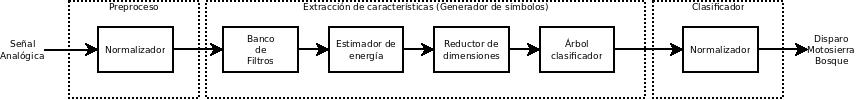
\includegraphics[width=\textwidth]{SiRPA.jpeg}
\centering
\caption{Diagrama de bloques del Sistema de Reconocimiento de Patrones Acústicos \cite{Carlosthesis}}
\label{sirpa}
\end{figure}


\section{Descripción del problema y justificación}

Como fue mencionado en el apartado anterior, países como Costa Rica ven amenazados sus recursos naturales por actividades ilegales como la caza furtiva y la tala. La tutela de los recursos naturales por parte del Estado es difícil, los bosques y los grandes mamíferos ven amenazada su conservación. En respuesta a esta situación la escuela de Ingeniería Electrónica del Instituto Tecnológico de Costa Rica, a través del \textit{DCILab} \footnote{DCILab: Laboratorio de Diseño de Circuitos Integrados} plantea una solución mediante un dispositivo electrónico de bajo consumo energético, capaz de reconocer sonidos como disparos de armas de fuego y motosierras. Esta iniciativa da a luz al proyecto SiRPA el cual pretende fabricar un \textit{ASIC} \footnote{ASIC es el acrónimo en inglés para: Circuito Integrado de Aplicación Especial... Se invita al lector a consultar un diccionario de términos electrónicos diccionario de términos electrónicos} con el fin de detectar la tala y caza ilegal en bosques, mediante el procesamiento digital de señales acústicas.

Luego de muchas etapas iterativas en el diseño del \textit{SiRPA}, el proyecto se encuentra codificado en un lenguaje de descripción de hardware (\textit{HDL}). Se han efectuado pruebas usando plataformas de sistemas embebidos como \textit{Beagle Boards} y textit{FPGAs} \footnotetext{Una FPGA (del inglés Field Programmable Gate Array) es un dispositivo electrónico que contiene bloques de lógica y electrónica digital que puede ser reconfigurada “in situ” mediante un lenguaje de descripción de hardware.} para la validación del diseño, se han publicado algunos papers al respecto, y se ha demostrado la viabilidad del proyecto, por lo que compete continuar la labor de
implementar la codificación \textit{HDL} a su etapa final, la cual consiste en la síntesis de los módulos
descritos en HDL sobre un chip de silicio.

Durante el 2014 el \textit{DCILab} contó con el apoyo del ingeniero argentino Dr. Juan Agustín Rodríguez, quien desarrolló un flujo de diseño digital sobre las herramientas de software Synopsys que implementan los módulos en HDL del \textit{SiRPA} al silicio para el circuito integrado. El trabajo del Dr.Rodríguez quedó incompleto y el \textit{SiRPA} no ha podido ser fabricado. Es por ello que el \textit{DCILab} requiere terminar el trabajo empezado por el Dr. Rodríguez e integrar la parte final del \textit{SiRPA}, que consiste en un microprocesador desarrollado por el Ing. M.Sc. Carlos Salazar García, para así dejar todo el proyecto \textit{SiRPA} depurado y listo para su fabricación. Además el \textit{DCILab} está interesado en que dicho proceso de síntesis quede documentado y se establezca una estructura de diseño digital genérica, capaz de ser adaptada para futuros proyectos.

Los investigadores del \textit{DCILab} logran fabricar sus circuitos integrados mediante el servicio de
“Obleas Multi-Proyectos” de \textit{MOSIS} \footnote{MOSIS (Metal Oxide Semiconductor Implementation Service): es un servicio que facilita servicios para la fabricación de circuitos integrados, como tal no es una fábrica, sólo un facilitador de tecnologías de fabricación.}. Este servicio lo brinda el Instituto de Ciencias de la
Información de la Universidad del Sur de California (USC). MOSIS consiste en un proyecto que ofrece
la opción para que pequeños diseñadores independientes, y instituciones académicas puedan fabricar
sus proyectos a un costo accesible y en una tecnología que se ajuste a sus requerimientos. \cite{website:mosis}

\section{Síntesis del problema}
El proyecto \textit{SiRPA} se encuentra inconcluso y el \textit{DCILab} requiere de una persona con conocimientos en microelectrónica capaz de someter los componentes del \textit{SiRPA} a un flujo de diseño \textit{ASIC}, y fabricar un prototipo \textit{SoC}.

\section{Enfoque de la solución}

\subsection{Generalidades de la solución}

Dado que se requiere diseñar un circuito integrado digital que parte de una codificación \textit{HDL}, es necesario desarrollar una jerarquía de diseño digital que permita realizar el layout de los módulos descritos en \textit{HDL}, por lo que se necesita de una herramienta de software especializada para tal fin. \textit{Design-Compiler} e \textit{IC-Compiler} son herramientas interactivas de \textit{Synopsys} que le permiten al usuario controlar el desarrollo del circuito integrado sobre el silicio, definiendo las características físicas como: conexión eléctrica, distribución espacial y física, limitaciones espaciales y sus implicaciones electromagnéticas para que su posterior fabricación e implementación física sean exitosas.

El proceso de diseño de un circuito integrado es lento, tedioso, y tiene un componente iterativo, esto implica que toma de algún tiempo para que un ingeniero se familiarice con el flujo de diseño, es por ello que aparte de crear el flujo de diseño de un chip sobre la herramientas, es conveniente establecer para futuros proyectos, una estructura de archivos y \textit{\textbf{scripts}}, propios de las herramientas de \textit{Synopsys}, para así facilitar el diseño y rediseño de proyectos futuros del \textit{DCILab}. Como comprobación de la efectividad del flujo de diseño digital anteriormente mencionado, deberán someterse los componentes del \textit{ASP} mediante las herramientas de  \textit{Synopsys}, para su posible fabricación a futuro, y establecer una documentación oportuna para agilizar el trabajo, de los colabores del \textit{DCILab} en cuanto a síntesis sobre silicio respecta.

\subsection{Síntesis de la solución}
Establecido el panorama anterior, la solución consiste en desarrollar una jerarquía de flujo de diseño digital en las herramientas de \textit{Synopsys}, que permita someter los componentes del \textit{SiRPA} al proceso de síntesis al silicio, según las reglas de diseño del proceso de fabricación de IBM: cmrf8 (IBM013), que es la tecnología a la cual
tiene acceso el \textit{DCILab}, y así contar con el proyecto \textit{SiRPA} completo hasta la última etapa previa a su fabricación que será realizada por \textit{MOSIS} en un futuro.
Cabe destacar que la índole del proyecto y las restricciones del laboratorio en términos de licencias de software solamente permiten una opción de \textit{EDA} \footnote{EDA: Electronic Design Automation. Software usado en la síntesis de circuitos integrados}, la cual es \textit{Synopsys}.

\section{Trabajos Anteriores}

\textit{SiRPA} es un proyecto de investigación que ha sido explorado y analizado desde diversas perspectivas de solución cada investigador ha dado forma a cada etapa que componen el sistema. Tanto a nivel de software como a nivel de hardware, los aportes incluyen desde propuestas de diseño, implementación, mejoras o rediseño de etapas que han presentado problemas. Entre estos trabajos se encuentran los siguientes:

\begin{itemize}

\item {En \cite{MSaenz}, se efectuó la primera prueba de concepto para evaluar la viabilidad de implementar el SiRPA. Se empleó el software MATLAB, para generar un modelo de alto nivel cuyo objetivo fue el análisis de las señales acústicas y se desarrolló una etapa de identificación de características utilizando la teoría de onditas (wavelets en ingles). Este trabajo constituye la primer referencia del sistema. La estrategia de extracción de características mediante onditas fue descartada posteriormente}

\item {En \cite{Esalas}, se implementó el \textit{SiRPA} en una \textit{FPGA} utilizando el lenguaje de descripción de hardware \textit{VHDL}, de este trabajo se establece que el uso de un banco de filtros utilizando una misma unidad de filtro para cada una de las ocho bandas constituye una metodología de clasificación idónea para los requerimientos de hardware del \textit{SiRPA}. Es en este trabajo donde se intenta implementar por primera vez el algoritmo de \textit{HMM} en hardware mediante un MAP (del ingles Matrix and Arrays Processor), el cual consiste una estructura digital cuya arquitectura se optimiza de acuerdo con la ejecución de operaciones en punto flotante en 32 bits de forma combinacional.}

\item {En \cite{Msequeira}, se desarrolló un módulo reductor de dimensiones mediante la estrategia de transformación lineal, fundamentada en el algoritmo de discriminantes de Fisher. Este módulo permite transformar un espacio de 8 dimensiones en un espacio de 3 dimensiones, que implica mayor facilidad en la clasificación de señales acústicas y ahorro energético, al disminuir la densidad de hardware.}

\item {En \cite{Jcardenas}, se desarrolló la herramienta HMMSoft que consiste en un software de alto nivel (lenguaje C/C++) con interfaz gráfica, capaz de realizar el entrenamiento del algoritmo de \textit{HMM} utilizado por el clasificador. Esta aplicación permite identificar características de patrones acústicos lo cual contribuye a validar el reconocimiento de un audio en particular. Esta herramienta representa un hito considerable ya que mediante ella, es posible establecer un marco de referencia para la verificación funcional del sistema.}

\item {En el trabajo de \cite{Jordanthesis}, se realizó la síntesis de la sección de extracción de los patrones acústicos y entrenamiento a partir de conjuntos de datos de audio similares a los que se esperara detectar. El proceso de extracción mencionado fue integrado a la aplicación HMMSoft \cite{Jcardenas}. Consecuentemente el proyecto \textit{SiRPA} fue modelado en el lenguaje C, e implementado en un sistema embebido (BeagleBoard xM)  \cite{website:beagleboard} y usando la herramienta HMMSoft además del modelo en C del \textit{SiRPA} se desarrolló el primer modelo de verficación para \textit{SiRPA}} 

\item {En \cite{Lalfaro}, se implementaron los módulos de hardware del reductor de dimensiones, generador de símbolos y una unidad de \textit{HMM} en \textit{Verilog}. Partiendo de la estructura de la unidad \textit{HMM} desarrollada por \cite{Jordanthesis} para el sistema embebido, en \cite{Lalfaro} se propone implemetar la unidad mediante una máquina microprogramada. Posteriormente al realizar pruebas sobre una FPGA, se observó que los resultados divergen de lo esperado según el modelo de \cite{Jordanthesis} y por tanto clasificar los patrones acústicos correctamente es imposible. Según expone \cite{Carlosthesis} el hardware presenta problemas de cálculo ya que los resultados tienden a cero rápidamente debido a que en \cite{Lalfaro}, no se consideran los problemas de escalamiento que se describen ámpliamente en \cite{LRabiner}.}

\item {En \cite{Mau}, se expone la verificación funcional de los módulos descritos en hardware (textit{HMM}) que conforman el SiRPA.}

\item {En \cite{mio}, se toma como punto de partida el trabajo de \cite{Esalas} y se rediseñó la unidad contemplando efectos de submuestreo. De acuerdo con un analisis del bloque de reducción de dimensiones elaborado en \cite{Lalfaro} se estableció la necesidad de aumentar el formato de palabra de 16 a 24 bits. Por lo tanto se integraron además todos los bloques para formar la etapa de identificación o extracción de características. Finalmente, se evaluó la funcionalidad de esta etapa, tomando como referencia dorada el trabajo realizado en \cite{Jordanthesis}.}

\item {En \cite{Carlosthesis} se expone la necesidad de implementar la unidad de clasificación \textit{HMM} mediante un microprocesador de aplicación específica ya que durante la experimentación en \cite{mio} se determinó que la unidad \textit{HMM} implementada en \cite{Lalfaro} no era correcta.}

\end{itemize}

\section{Objetivos}

\subsection{Meta}

Desarrollar un sistema de detección de disparos de armas de fuego, motosierras y otras actividades ilegales en un bosque, que esté implementado en un circuito integrado de bajo consumo energético.

\subsection{Objetivo General}

Implementar un microprocesador de aplicación específica en una tecnología CMOS de 0,13 micrómetros para posteriormente ser integrado al proyecto SiRPA.


\subsection{Objetivos Específicos}

\begin{itemize}

\item{Diseñar una jerarquía de scripting \footnote{En informática un script es un archivo que contiene un conjunto de órdenes e instrucciones, las cuales ejecutan una función, ya sea en un lenguaje de programación o una herramienta de software. Se invita al lector a consultar un diccionario de términos de computación} que implemente el flujo de síntesis y simulaciones {"Post Colocado y Enrutamiento"} (Place\&Route), para optimizar el tiempo del proceso de diseño para futuros proyectos.}

\item {Sintetizar lógicamente de manera correcta los módulos RTL del Microprocesador de Aplicación Específica (ASP) sobre celdas estándar de una tecnología CMOS 0,13.}

\item {Sintetizar físicamente de manera correcta la unidad aritmética del microprocesador y la memoria de programa del microprocesador ASP sobre la tecnología CMOS 0,13}

\end{itemize}
%%% Local Variables: 
%%% mode: latex
%%% TeX-master: "main"
%%% End: 

  \chapter{Marco Teórico}
\label{ch:marco}
\subsection*{Diseño de ASICs}

{Esta tesis no pretende exponer el proceso de fabricación de un circuito integrado, esa información puede encontrarse en un libro de texto sobre diseño VLSI; sin embargo, en las secciones siguientes se expondrá brevemente, la metodología que se esta usando para que a futuro se pueda llevar a cabo la implementación de un sistema sobre un dado de silicio (silicon dice), entendiendo por dado el espacio que el sistema propuesto ocupará sobre la oblea de silicio, al final del proceso de fabricación.

Comercialmente la manufacturación de ASICs no es rentable para aplicaciones de envergadura pequeña, ya que un proceso de fabricación fácilmente alcanza los millones de dolares, si se tiene una proyección comercial baja o nula esta opción queda descartada, la forma más fácil de implementar un diseño en un chip sería venderle la idea o diseño a un fabricante.

No obstante, venderle la idea o diseño a un fabricante implica revelar información sensible sobre el producto y el fabricante probablemente este trabajando con su competencia por lo que revelarle su trabajo a un fabricante tampoco es la mejor opción.

Sin embargo, es posible hacer el proceso de diseño, posteriormente generar un archivo que contenga toda la información estrictamente necesaria para que el fabricante pueda implementar el diseño sobre el chip, sin tener revelar la información sensible que se pretende proteger.

Esta suele ser la opción más viable para los pequeños investigadores; no obstante, existe la problemática que este tipo de servicio alcanza precios muy elevados sobre todo si se pretende emplear los procesos más modernos y las tecnologías de vanguardia.

En respuesta a la problemática de no tener suficientes fondos para concretar una fabricación, existe el servicio de óbleas multiproposito de la universidad de Berkeley (\textit{MOSIS}).

La funcionalidad de implementar sistemas sobre chips (SoC) tiene grandes ventajas respecto a sistemas embebidos o implementados mediante software de alto nivel.

En primera instancia producir un sistema en un circuito integrado representa una mejor protección para los derechos intelectuales, pues su contenido difícilmente es reproducible. Un circuito integrado presenta enormes facilidades de portabilidad debido a su tamaño y su consumo energético. Lo cual es el principal objetivo del proyecto: "Sonidos Ilegales".

\subsection*{Sobre la tecnología de fabricación}

Para el presente proyecto se hace uso de la tecnología de IBM CMOS8RF (CMRF8SF), esta tecnología cuenta con una alta densidad de lógica CMOS de  0.13 $\mu$m destinada a aplicaciones de señal mixta, en ámbitos asociados al procesamiento analógico y de radio frecuencia . Entre las generalidades del proceso, cabe destacar que cuenta con 8 capas de metal, y la tensión $V_{DD}$ de los dispositivos se encuentra en un rango de 1.2 V a 1.5 V.\\

\section{Tipos de diseño circuitos integrados digitales}

La clasificación del diseño de circuitos integrados se puede apreciar en el esquema de la figura \ref{ICs}.

\begin{figure}[h]
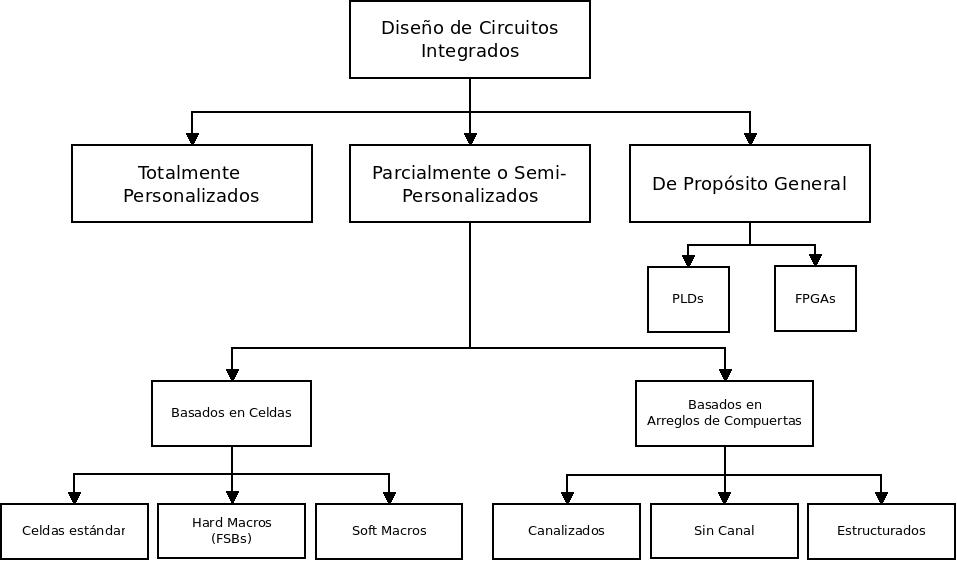
\includegraphics[width=\textwidth]{Tipos_de_ICs.jpeg}
\centering
\caption{Tipos de Diseño de Circuitos Integrados}
\label{ICs}
\end{figure}
Como podemos observar el diseño de circuitos integrados (De aquí en adelante ICs\footnote{ICs: acrónimo en inglés para circuitos integrados}) se puede clasificar a grosso modo en 3 tipos principales:

\subsection{\textbf{ICs totalmente personalizados}}

En esta metodología de trabajo los diseñadores generan todas las celdas lógicas de acuerdo con las necesidades tiene el diseño que se pretende realizar, esto contempla desde la concepción funcional, lógica y física de cada celda. También se desarrollan las máscaras necesarias para la fabricación del chip sobre la oblea de silicio.

Empresas como Intel son un buen ejemplo de industrias dedicadas al desarrollo de circuitos integrados totalmente personalizados, aquí los ingenieros invierten enormes cantidades de tiempo maximizando el aprovechamiento de cada micrómetro cuadrado disponible en el dado, lo que les permite incluir circuitos analógicos, optimizar celdas de memoria e incluso contemplar y mejorar la eficiencia mecánica de las estructuras de conexión y ubicación de los componentes del chip.

Sin duda la metodología más costosa de todas. No obstante, la respuesta adecuada si el diseñador necesita de unidades (celdas) más eficientes en términos energéticos y velocidad, de las que es capaz de encontrar en una biblioteca de celdas existentes. Es comúnmente utilizada por empresas dedicadas a la innovación y el desarrollo tecnológico.

\subsection{\textbf{ICs programables}}

Estos consisten en dispositivos lógicos programables (PLDs), que son circuitos integrados con configuraciones estándar, predeterminadas. Podemos encontrarlos en algunos ASICs para permitir la personalización de algunas funciones puntuales, es por ello que aunque sean estructuras prediseñadas y flexibles, son consideradas como una rama del diseño de ICs.

\subsection{\textbf{ICs semipersonalizados}}

Son aquellos ICs para los cuales existe una biblioteca de celdas estándar y posiblemente todas las mascaras de diseño están disponibles. El uso de bibliotecas de celdas prediseñadas hace el diseño más fácil. Está metodología de diseño se subdivide en dos partes:

\subsubsection{Basado en arreglos de compuertas}

En este tipo de diseño los transistores se encuentran predefinidos en un patrón dado sobre en la oblea de silicio, este patrón se conoce como arreglo base y a los elementos más pequeños se los conoce como celdas base o celdas primitivas.

En esta técnica el diseñador únicamente define la interconexión de las celdas usando para ello máscaras personalizadas. Así el diseñador escoge de entre una basta biblioteca de celdas prediseñadas y precaracterizadas. Las celdas lógicas suelen ser denominadas como macros. La razón de esto se debe a que el layout \footnote{En este contexto, refiere al anglisismo asociado al concepto de diseño físico} de la celda base es el mismo para cada celda lógica y únicamente se personaliza la interconexión y el enrutado dentro de las celdas y con las celdas adyacentes, de manera similar a un macro de software.

Existen subcategorias del uso de esta técnica, pero esa información excede el alcance de esta tésis, por lo que no serán expuestas. Se invita al lector a considerar una bibliografía pertinente \cite{book:johnM1997,book:barrK2006}

\subsubsection{Basado en celdas estándar}

Un circuito integrado basado en celdas estándar usa celdas lógicas prediseñadas como compuertas "Y", "O", "Flip Flops", "Multiplexores", etc... Estas celdas se conocen como celdas estándar.

Suele usarse el término \textit{CBIC} (pronunciado si-bik) para esta categoría. El área de ubicación de las celdas estándar en un \textit{CBIC}, se construye en hileras, de manera similar a una pared de ladrillos, las celdas estándar pueden y suelen ser utilizadas en conjunto a microcontroladores, o microprocesadores, conocidos como "Mega celdas". Este término también se emplea para bloques totalmente personalizados, y suelen ser denominados como: "Macros a Nivel de Sistema (SLMs)", "Mega Funciones", "Bloques Fijos", o "Bloques Funcionales Estándar (FSBs)".

En esta metodología es diseñador define únicamente la colocación y el enrutado (interconexión entre celdas estándar) de las celdas estándar; sin embargo, estás pueden ser colocadas libremente en el área disponible del dado. Esto implica que las máscaras de fabricación en un \textit{CBIC} son únicas para cada cliente.

Usar \textit{CBICs} tiene enormes ventajas ya que permite hacer diseños más flexibles y optimizarlos en términos de aprovechamiento de área, velocidad o consumo energético. Adicionalmente las bibliotecas de celdas estándar suelen ofrecer las mismas celdas estándar prediseñadas para cumplir distintas las expectativas de desempeño, enfocadas a tamaño, velocidad o energía.

Las principales desventajas consisten en que el tiempo necesario para el diseño suele ser elevado, debe comprarse una biblioteca de celdas estándar, y se está sujeto a las restricciones de esta, y finalmente las máscaras de fabricación serán nuevas con cada nuevo diseño o versión de diseño, lo cual implica tiempo adicional, además de costos adicionales por parte del fabricante.

La información de esta sección se tomó a partir de las fuentes \cite{book:raj2008,book:johnM1997,book:raj2008}

\section{Flujo de diseño digital para el diseño de circuitos integrados digitales}

Dada la complejidad en el proceso de diseño de circuitos integrados, es imperativo llevar a cabo un diseño estructurado, que use los principios de jerarquización, modularidad, regularidad y localidad para manejar la complejidad del diseño.

El diseño digital VLSI suele ser particionado en 5 niveles de abstracción: diseño de arquitecturas, diseño de microarquitecturas, diseño lógico, diseño de circuitos y diseño físico. Estas etapas son ejecutadas en paralelo, y en muchas ocasiones son depedientes entre si.

Una manera alternativa de analizar el diseño estructurado es mediante el "diagrama Y" mostrado en la figura \ref{Ychart}. 

\begin{figure}[h]
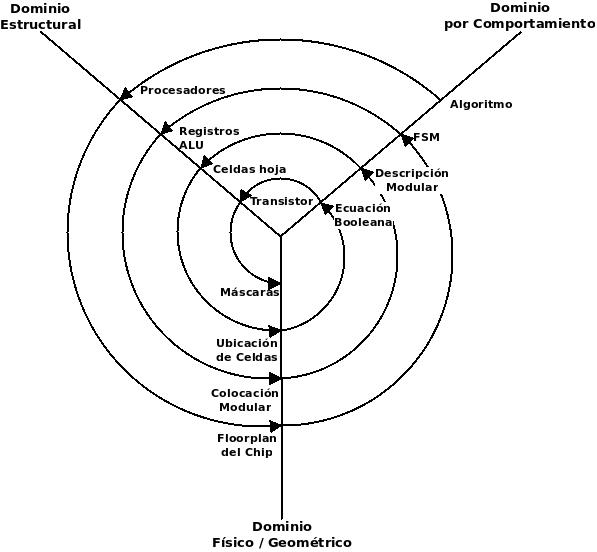
\includegraphics[width=\textwidth]{Gajski_Y_Chart.jpeg}
\centering
\caption{Diagrama de Gajski. Espiral que ilustra el flujo digital de diseño de circuitos integrados y cuyas arístas establecen los ámbitos por los que debe atravesar el diseño. Figura de autoría propia, basada en la reproducción de \cite{book:weste2005}, créditos a sus respectivos dueños}
\label{Ychart}
\end{figure}

El diagrama de Gajski o diagrama Y, permite entender el concepto de abstracción en el diseño digital, pues se parte desde un concepto general de diseño y al interiorizar en el diagrama se desvelan las etapas que llevan hasta la fabricación correcta del circuito integrado.

El dominio por comportamiento describe qué hace el sistema, seguidamente en el dominio estructural, el cual expone la interconexión de los módulos capaces de realizar el comportamiento deseado, eventualmente a los niveles de abstracción más bajos donde se describen las compuertas individuales y las conexiones entre los transistores que las componen. Finalmente en cada nivel de abstracción del dominio físico se explica como se construye físicamente ese nivel de abstracción, en los niveles más altos se considera el diseño del floorplan del chip, donde en esencia se , y consecuentemente al internarse en los niveles más profundos se describen la geometría actual de cada transistor individual.

El proceso de diseño puede verse como la transformación desde un dominio hacia otro manteniendo la equivalencia de los dominios. Las descripciones por comportamiento se transforman en descripciones estructurales y estas a su vez son transformadas en descripciones físicas. Cada transformación es validada, ya sea manualmente o mediante herramientas automatizadas. La especificación jerárquica de cada dominio y sucesivamente detallando sus niveles de abstracción es lo que permite diseñar grandes sistemas. 

La razón para describir en detalle los niveles de abstracción y los respectivos dominios es para definir un proceso de diseño en el cual la función final del sistema es capaz de rastrearse hasta la descripción por comportamiento inicial.

El diagrama Y muestra las transformaciones entre cada dominio y las variaciones entre los niveles de abstracción. El flujo de diseño procede desde los anillos exteriores hacia los interiores, profundizando en niveles de abstracción cada vez más complejos, de acuerdo a una jerarquía establecida.

El apartado anterior corresponde a una libre interpretación de la sección 1.6 de \cite{book:weste2005}.

\subsection{Generalidades del flujo de diseño digital}
\label{sec:gen_d_flow}
\begin{figure}[t]
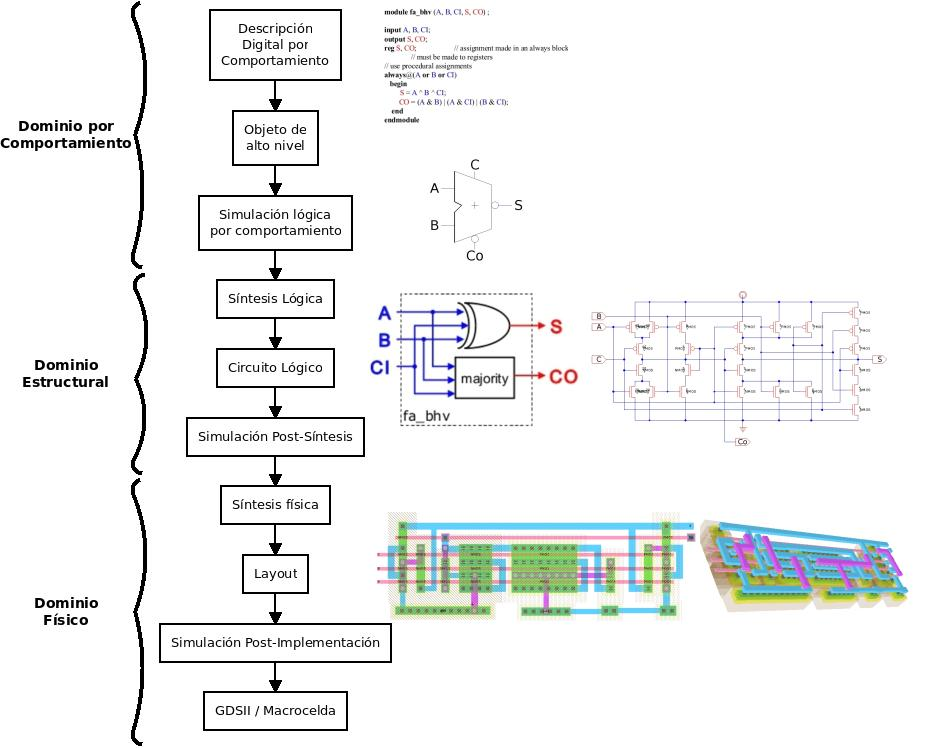
\includegraphics[width=\textwidth]{Flujo_Digital.jpeg}
\centering
\caption{Esquema representativo e ilustrativo del flujo de diseño de circuitos integrados digitales}
\label{Dflow1}
\end{figure}

Como se mencionó en el apartado anterior, el diseño comienza a dar sus pasos en cuanto es concebida una función o proceso y su comportamiento ha sido modelada en un algoritmo, ya sea secuencial, concurrente o una mezcla de ambos. Este algoritmo se traduce a un lenguaje estandarizado, el cual en el caso de los circuitos integrados digitales corresponde a un \textit{HDL}, que en términos concretos es la descripción digital del circuito integrado o el modelo digital.

Partiendo del modelo digital se puede hacer una verificación de comportamiento, que en términos técnicos se denomina simulación lógica, el modelo digital no es más que un objeto de alto nivel capaz de emular el comportamiento deseado. Su utilidad es poca para el diseñador, ya que no provee datos sobre el desempeño del diseño, únicamente provee 
información a nivel de comportamiento; sin embargo, es el punto de partida en el flujo de diseño.

Una vez que la simulación lógica es satisfactoria, se procede a usar el modelo por comportamiento y asociar los módulos descritos en él, con unidades lógicas provistas de características de retardos (sincronización de señales), consumo energético, y área, las cuales se encuentran en la biblioteca de la tecnología que se usará en la fabricación. A este proceso se le conoce como síntesis lógica, y genera una base de datos que contiene datos de las celdas estándar y las conexiones entre ellas para ejecutar las funciones abstraídas del modelo de comportamiento.

La base de datos creada en el proceso de síntesis permite generar un nuevo modelo codificado en \textit{HDL} y una primera aproximación del desempeño de los módulos diseñados, i.e. un modelo con la información sobre los retardos de propagación de las señales en las celdas y entre las mismas, generar un presupuesto de la energía disipada y el área necesaria para ubicar las celdas usadas. Este nuevo modelo, denominado como modelo post-síntesis nuevamente es simulado con el mismo arreglo o banco de pruebas usado en la simulación por comportamiento.

La simulación post-síntesis permite observar el retardo de propagación de las señales, y confirmar si las expectativas de sincronización son alcanzadas, también permite verificar si los datos son generados en los plazos necesarios, y poder garantizar una funcionalidad correcta de los módulos y el diseño en lo concerniente al desempeño de las celdas estándar. 

Cuando los resultados obtenidos en la síntesis lógica y la simulación respectiva sean satisfactorios, se toma el modelo post-síntesis y se usa esta información para empezar con el floorplan del chip. Las celdas estándar son invocadas a un área determinada, y posteriormente se establecen las conexiones que permiten implementar los módulos abstraídos en la primera etapa del diseño (el modelo de comportamiento). Este proceso recibe el nombre de síntesis física o implementación física, en esta tésis se usará la palabra síntesis para referirse a la síntesis lógica, y la palabra implementación será usada para referirse a la síntesis física.

Una vez hecho lo anterior, se genera una nueva base de datos, la cual tendrá información más precisa sobre el diseño, nuevamente en términos de sincronización de señales, consumo energético y aprovechamiento de área, incluyendo los retardos debido a los efectos parasíticos, la distancia que debe recorrer una señal al conectarse de una celda a otra o un puerto, etc, las perdidas resistivas del alambrado, entre otros efectos que serán expuestos más adelante.

Nuevamente se genera una base de datos con la información del colocamiento y el enrutado (Place\&Route), así como los efectos sobre el tiempo de propagación de las señales, mediante la esta base de datos se generan, un modelo codificado en \textit{HDL} para la verificación del diseño, y el modelo de los efectos sobre el temporizado y la sincronización de las señales. En esta etapa es posible obtener una respuesta más precisa del diseño. Al igual que en la etapa anterior también se crean reportes de consumo energético, aprovechamiento de área, calidad de resultados, etc.

Cuando una simulación post-implementación es satisfactoria se procede a dar por concluído el flujo, y a continuación se establecen 2 panorámas.

En el primer caso nuestro diseño está completo por lo que se procede a compilar la base de datos en un archivo estándar para condensar la información necesaria para el fabricante, y este valorará si el diseño tiene probabilidades altas de ser fabricado con éxito, siendo así la información suministrada será usada para desarrollar las máscaras necesarias para la construcción del chip.

En el segundo escenario consiste en que el diseño en el que se ha estado trabajando no es el producto final, sino que forma parte de otro diseño más complejo y grande, el cual aún no se haya terminado, en ese caso la base de datos servirá para generar una macro celda que será utilizada en diseños posteriores.

En la figura \ref{Dflow1} se aprecia un resumen gráfico de la explicación anterior.

\subsection{Flujo de diseño digital en las herramientas de Synopsys}

Synopsys es una empresa que brinda herramientas de diseño asistido por computadora (CAD), para la automatización de procesos en el diseño de circuitos integrados. El flujo de diseño digital suele ser similar independientemente del proveedor de las herramientas; sin embargo, esta tesis gira entorno a los softwares de Synopsys, por lo que se expondrá la metodología de diseño usando este proveedor.

\subsection{Front End}

\begin{figure}[h]
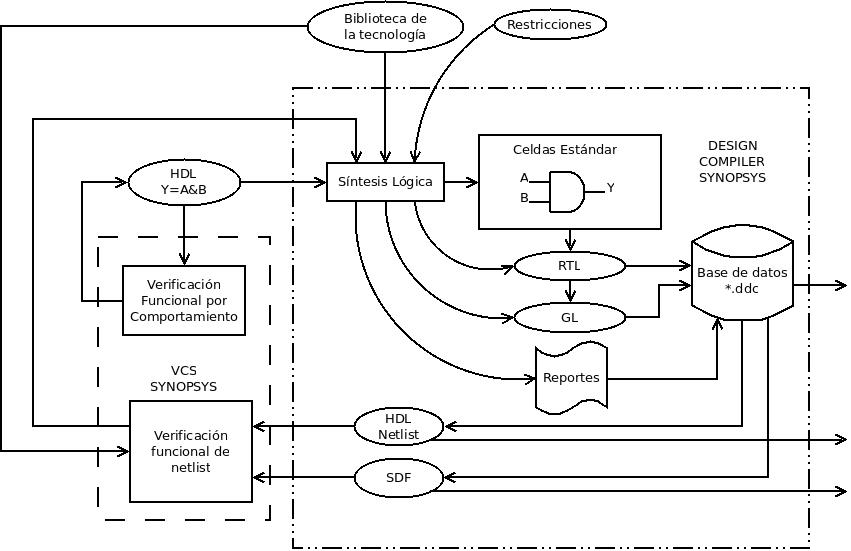
\includegraphics[width=\textwidth]{Front_End.jpeg}
\centering
\caption{Esquema ilustrativo del flujo de diseño de circuitos integrados digitales, enfocado a las herramientas de síntesis lógica, en esencia las herramientas de Front End}
\label{fe}
\end{figure}


El término "Front End", es un concepto en inglés asociado a la jerga del desarrollo de software, y significa interfaz; sin embargo, en el caso del diseño de circuitos integrados, no se generan softwares y tampoco interfaces. Una traducción más literal, y por lo tanto, menos elegante del concepto sería "Fachada", y es en esencia con lo que el diseñador interactúa en la primer etapa del diseño.

Al decir que el diseñador interactúa con una fachada, se debe entender que el diseñador trabaja con el cascarón de un elemento que intrínsecamente no es circuito electrónico como tal, si no un modelo abstracto que presenta un comportamiento de causa efecto, el cual, naturalmente, es acorde a la semántica de la lógica digital, o lógica binaria. Recurriendo nuevamente a la jerga del software, podemos entender el front end o fachada como aquello relacionado con un objeto de alto nivel, que ofrece un vector de respuestas de acuerdo con la dinámica de un vector de estímulos.

El diseñador comienza a acercarse al diseño del circuito integrado, considerando y definiendo los aspectos principales de la fachada. Retomando el diagrama de Gajski (figura \ref{Ychart}), el proceso de "Front-End" consiste en la transición del modelo de comportamiento a un modelo estructurado, que se asocia con las funciones de las celdas estándar ofrecidas por la tecnología y el fabricante.

Condensando lo anterior, las herramientas de "Front-End" de un proveedor, son aquellas que ejecutan o facilitan el proceso de síntesis lógica en el flujo digital del diseño de circuitos integrados. En el caso de "Synopsys", estas herramientas son principalmente "Design Compiler" y "VCS", existen otras herramientas adicionales asociadas a la familia de "Design Compiler", "VCS" y el "Shell" de "Design Compiler" son las principales y suelen ser suficientes.

En la figura \ref{fe} se aprecia un diagrama que ilustra como el proceso expuesto en la sección \ref{sec:gen_d_flow}, es implementado por las herramientas de "Synopsys" todos los procesos en el diseño de circuitos integrados tienen un componente iterativo, y en este diagrama vemos como antes de avanzar en el flujo, se atraviesa por etapas a las que se recurre con frecuencia, estas etapas son las simulaciones por comportamiento y post-síntesis. La depuración de la etapa de síntesis es esencial para garantizar el éxito final del proyecto, por lo que las simulaciones tienen una gran importancia.

Cómo se observa desde el diagrama de Gajski (figura \ref{Ychart}), las herramientas de "front end" traducen el diseño por comportamiento en modelos de altos nivel de circuitos digitales, aunque como tal no se trabajan con circuitos lógicos reales, y para efectos prácticos el diseñador nunca trabaja realmente con elementos lógicos y digitales, las herramientas proveen la virtualización del comportamiento diseñado, mediante una biblioteca de simulación, las celdas estándar abstraídas en el proceso de síntesis, se comportarán como un elemento de circuito digital real, de ahí que se pueda validar si la etapa de síntesis cumple las expectativas del diseñador.

\newpage
\subsection{Back End}

\begin{figure}[h]
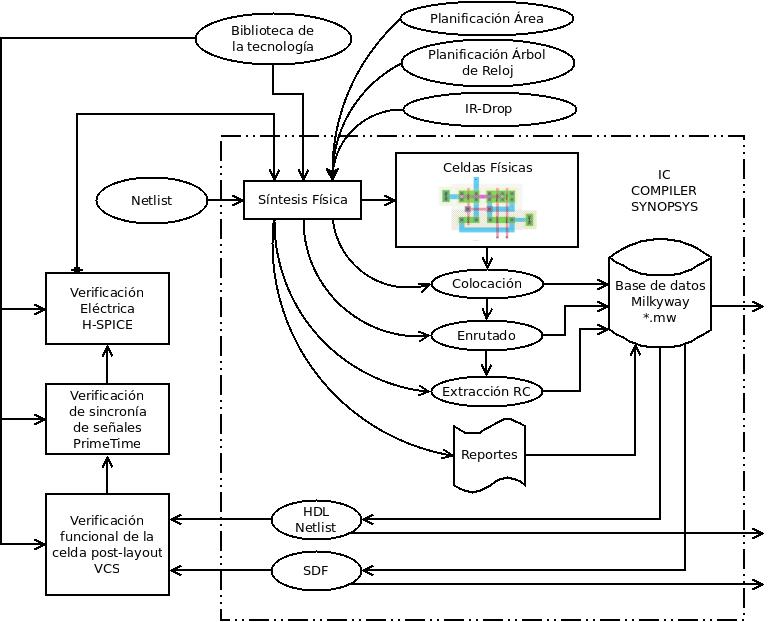
\includegraphics[width=\textwidth]{Back_End.jpeg}
\centering
\caption{Esquema ilustrativo del flujo de diseño de circuitos integrados digitales, enfocado a las herramientas de síntesis lógica, en esencia las herramientas de Front End}
\label{be}
\end{figure}

Se refiere a aquellos procedimientos relacionados con la constitución interna de un proyecto, nuevamente se emplea el anglicismo "Back End" para referirse a dichos procesos. No existe un concepto en español capaz de traducir el significado de esta palabra, pero se podría entender como todos aquellos aspectos ocultos al macro diseñador, entendiendo por oculto, una serie de elementos compuestos por elementos más simples hasta llegar a las unidades fundamentales de la electrónica moderna, i.e. transistores. Una analogía curiosa, y que ilustra bien esta situación es la de la muñeca matryoshka \cite{book:matryoshka}, cada muñeca contiene a otra muñeca más pequeña, y se interioriza así hasta alcanzar una pequeña muñeca que no contiene a ninguna otra.

En el proceso de diseño de circuitos integrados, semipersonalizados, y basados en celdas estándar, el diseñador no alcanza a trabajar directamente con transistores, o con los elementos que componen las celdas, si no, que da por hecho que las celdas estándar son funcionales y parte de ellas para generar nuevas macroceldas, y con las cuales se ejecutarán las funciones establecidas por el macromodelado del funcionamento del diseño.

En síntesis de lo anterior, el diseñador de "back end" trabaja con las etapas ocultas para los diseñadores de comportamiento, y síntesis del diseño, dónde los primeros establecen la semántica del diseño, y los segundos generan cajas negras que realizan las funciones descritas por sus antecesores, estas cajas negras manifiestan el comportamiento de una unidad electrónica real, en términos de consumo energético, área, y tiempos de propagación de señales, pero no dejan de ser modelos de alto nivel que no son circuitos electrónicos como tales, y es por ello que ha esta etapa se le denomina fachada.

En el proceso de "back end" las cajas negras abstraídas en el proceso de síntesis adquieren información más realista y equivalente a la de una celda física real. Esto podemos apreciarlo en la figura \ref{Dflow1} en el extremo derecho de la figura vemos como se muestran las etapas del flujo, en el dominio estructural, donde operan las herramientas de síntesis, aquí se muestran los bloques funcionales a nivel lógico. Al descender en el flujo expuesto en la misma figura, observamos la celda estándar que se abstrae del diseño estructurado, y su layout o implementación física, donde se aprecian los metales que interconectan las celdas y los transistores que componen las celdas.

Las herramientas de "back end" se encargan de facilitar el colocado y enrutado de las celdas estándar que se abstrajeron de la síntesis lógica. En el "back end" se asocia la base de datos post síntesis con la base de datos de la tecnología, invocando celdas físicas para generar un nuevo layout que implemente el diseño sintetizado. "Synopsys" cuenta con una herramienta llamada "IC Compiler", este software le permite al diseñador establecer los criterios de optimización del layout en términos de aprovechamiento de área, colocación selectiva para mejorar la eficiencia del consumo energético, sincronización de señales críticas, como lo es una señal de reloj, definir criterios de alambrado (enrutado) para sopesar las pérdidas resistivas, controlar fenómenos de electromigración y radiación o antena.





  \chapter{Solución propuesta}
\label{ch:solucion}

Primero que todo, jamás utilice el título indicado arriba, sino algo
relacionado con su solución: ``Sistema de corrección de distorsión'' o lo que
competa a su tesis en particular.

Este capítulo puede separarse en varias secciones, dependiendo del problema
concreto. Aquí los algoritmos o el diseño del sistema deben quedar lo
suficientemente claros para que otra persona pueda re-implementar al sistema
propuesto. Sin embargo, el enfoque no debe nunca concentrarse en los detalles
de la implementación particular realizada, sino del diseño conceptual como tal.

Recuerdese que toda figura y tabla deben estar referenciadas en el texto.

  \chapter{Resultados y Análisis}

En tesis formales en este capítulo se exponen los diseños experimentales
realizados para comprobar el funcionamiento correcto del sistema. Por ejemplo,
si se realiza algún sistema con reconocimiento de patrones, usualmente esta
sección involucra las llamadas \emph{matrices de confusión} donde se compactan
las estadísticas de reconocimiento alcanzadas. En circuitos de hardware,
experimentos para determinar variaciones contra ruido, etc. También pueden
ilustrarse algunos resultados concretos como ejemplo del funcionamiento de los
algoritmos. Puede mostrar por medio de experimentos ventajas, desventajas,
desempeño de su algoritmo, o comparaciones con otros algoritmos.

Recuerde que debe minimizar los ``saltos'' que el lector deba hacer en su
documento. Por tanto, usualmente el análisis se coloca junto a tablas y figuras
presentadas, y debe tener un orden de tal modo que se observe cómo los
objetivos específicos y el objetivo general del proyecto se han cumplido.

  \chapter{Conclusiones y Recomendaciones}

\section{Conclusiones}
Partiendo de una estructura básica para la integración de diseños codificados en RTL se ha logrado diseñar una jerarquía de archivos y directorios que permite implementar exitosamente un flujo de diseño de circuitos integrados digitales.

Mediante el uso de esta jerárquía fue posible implementar una unidad aritmética de punto flotante y demostrar que es correcta y funcional. Así mismo se demostró que es posible incorporar \textit{IP Cores} dentro del diseño y que los mismos son correctos y funcionales.

Debido a particularidades que se escapan de la visión de este trabajo no fue posible demostrar la funcionalidad del microprocesador RISC-V. Debido a deficiencias en la estructura de su RTL, sin embargo, quedó demostrado que el flujo es eficaz y eficiente.

Realizar una evaluación cuantitativa sobre la estructura de \textit{scripting} diseñada no es posible ya que responde a la visión de una única persona, y su paradigma particular de trabajo. Sin embargo, desde una perspectiva cualitativa y subjetiva, se considera la estructura de \textit{scripting} eficiente, pues manifiesta atributos como: regularidad, localidad y continuidad.

\section{Recomendaciones}

Se recomienda realizar una iteración en el diseño del microprocesador ASP, enfocado a incorporar una unidad para la programación de las memorias y permitir el \textit{booteo} del microprocesador.

Finalmente recomienda incorporar en una iteración futura optimizaciones asociadas con el área y la potencia de los módulos, incorporando técnicas como \textit{clock gating}, las cuales no fueron utilizadas en este proyecto.

  %----------------------------------------------------------------------------
  % literature
  \bibliographystyle{sty/plainurl} % for english documents
  \bibliography{literatura}
  %----------------------------------------------------------------------------

  %----------------------------------------------------------------------------
  \appendix
  %----------------------------------------------------------------------------

  \chapter{Hoja de Información del Proyecto}

% El título anterior es solo un ejemplo ilustrativo.  Éste teorema no ameritaría
% un apéndice pues es parte normal del currículum de Electrónica, pero apéndices
% usualmente involucran aspectos de esta índole, que se salen de la línea de la
% tesis, pero que es conveniente incluir por completitud.

% Los anexos contienen toda información adicional que se considere pertinente
% agregar, como manuales de usuario, demostraciones matemáticas que se salen de
% la línea principal de la tesis, pero que pueden considerarse parte de los
% resultados del trabajo.


  %----------------------------------------------------------------------------
  \backmatter
  %----------------------------------------------------------------------------

  \printindex                % insert index into document. Don't forget to call
                             % "makeindex filename" first.
\end{document}
